
\section{Simple data types}
\label{sec:simple-data-types}

Programs have lots of data, they are basically
ways of getting data, transforming data, and giving data back to the
world. 
%
A data type, as we have already seen, tell you which kinds of data you
have in your program. 

Simple data types can be thought as boxes in the computer's
memory. Every time you declare a variable in your program, you can
think\footnote{This is only a metaphore and is not supposed to be an
  accurate description of how memory is managed on a modern
  computer. Explaining how things like the registers, the stack, and
  the heap work, the differences between actual machines and virtual
  machines, etc; are out of the scope of this document.} of the
computer as creating a little box in its memory to store your
variable. That box has two tags on it: one of them holds the name of
the variable and the other holds the type
(Figure~\ref{fig:github}). In the same way, you can think of
assignment as putting a value inside that box. 

\begin{figure}
  \centering
  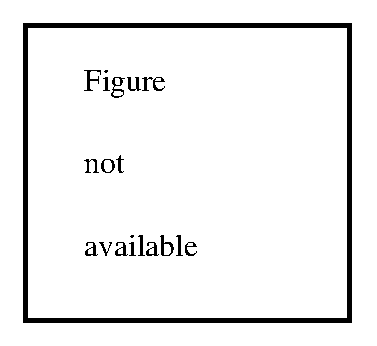
\includegraphics{gfx/no_figure}
  \caption{Declaring a variable in Groovy can be seen as creating a
    box. The box has a tag for the name and another for the type.}
  \label{fig:var1}
\end{figure}

\begin{figure}
  \centering
  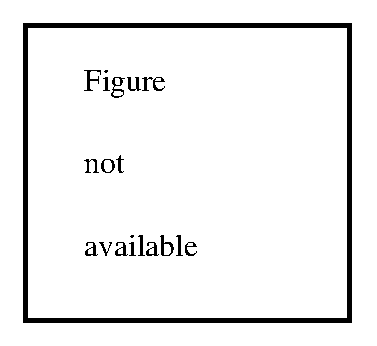
\includegraphics{gfx/no_figure}
  \caption{Assigning a value to a variable can be seen as putting a
    value in the box.}
  \label{fig:var1}
\end{figure}

\subsection{Static typing and dynamic typing}
\label{sec:strong-typing-weak}

You have already seen that Groovy, as most languages, puts some
restrictions to what you can use as a ``name'' tag for your boxes. You
know that they have to start with a letter: ``count'' is a valid name
but ``/me'' or ``5thNumber'' are not. You also know that some words
cannot be used by the programmer for variables names because it would
be confusing, e.g. ``while'', ``if'', ``System'', or ``println''.

Many programming languages also place one restriction on the ``type''
tag: once you decide the type of a variable, you cannot change
it. This is like people having static opinions that they do not want
to change. This type of languages are called \emph{statically typed
  languages} and, contrary to people with fixed ideas, they are
not necessarily bad or obnoxious. Java is an example of
statically typed language. 

Some programming languages allow you to change the type of your
variables as you go along, so you can have a variable that sometimes
is an int and later in time is a boolean or a String. These languages
are called \emph{dynamically typed languages}. They have pros and cons
compared to their statically typed counterparts. Groovy is an example
of a dynamically typed language. The following code excerpt is valid
in Groovy but not in Java. In Java a variable cannot be a String, and
then a boolean, and then a String again. Note that \emph{true} is a
boolean while \emph{``true''} (in quotes) is a String. 

\begin{verbatim}
    String str = "This is a string";
    str = true;   // This is different to: str = "true"
    if (str) {
      str = "This is a different string";
    }
\end{verbatim}

There are many more things to know about typing in programming
languages (strong vs. weak, inferred vs. manifest, duck typing, and
much more) but for now it will not be necessary to go into those
details. 

\subsection{Most common simple types}
\label{sec:most-common-simple}

\subsubsection{Integer numbers}
\label{sec:integers}

\subsubsection{Floating-point (decimal/rational) numbers}
\label{sec:float-point-decim}

\subsubsection{Boolean (binary) values}
\label{sec:bool-binary-valu}

\subsubsection{Characters}
\label{sec:characters}



% ...

You may have noticed that we have not mentioned String yet. This is
because String is a complex type. 

\section{Complex types}
\label{sec:complex-types}




%%% Local Variables:
%%% mode: latex
%%% TeX-master: "main"
%%% End:
